%% sections/results.tex — single-partition version
%% NOTE: all numbers in the tables are generated by make_tables_single.py
\section{Results}
\label{sec:results}

All results are from a single 10-fold cross-validation partition of the 247-patient discovery cohort
(natural patient order, the evaluation protocol of the original DyAM publication). Because one partition
can favour any model by chance, differences of the size reported below are described by direction and
magnitude, and the confidence intervals reflect patient sampling only.

\subsection{Multimodal Fusion Outperforms Single-Modality Baselines}
\label{sec:baselines}

Within the DyAM framework, models restricted to a single data source achieved AUC values of
$0.615$ (TMB), $0.606$ (pathology IHC-A), $0.701$ (CT radiomics), $0.676$ (genomics), and
$0.708$ (PD-L1~TPS) on the discovery cohort.
PD-L1~TPS was the strongest individual predictor among the biomarkers of routine clinical use,
although CT radiomics was comparable.

Fusing four data sources (CT radiomics, pathology IHC-A, genomics, and PD-L1~TPS) raised the AUC to
$0.798$ under the cooperative attention of the original framework, exceeding the best single source by
$0.090$~AUC; with IHC-G in place of IHC-A the four-source model reached $0.783$ (95\% CI 0.714--0.853),
and adding NLP-encoded clinical variables raised the latter to $0.803$ (0.738--0.868) (Table~\ref{tab:ovo_all21}).
Multimodal fusion is therefore the primary driver of predictive performance in this cohort, with no
individual source approaching the discrimination of the fused model.

%% ═══════════════════════════════════════════════════════════════════════════
%% B8 — NLP AUC Analysis
%% ═══════════════════════════════════════════════════════════════════════════

\subsection{NLP Encoding Improves AUC over Numeric Clinical Labs}
\label{sec:nlp_auc}

Seven clinical-encoding variants were evaluated under the DyAM architecture in two pathology
arms (IHC-A: seven variants; IHC-G: four variants)
(Tables~\ref{tab:auc_ihca} and \ref{tab:auc_ihcg}; Figure~\ref{fig:auc_comparison}).
Relative to numeric labs, the NLP raw (384-dimensional) encoding raised the AUC by
$+0.018$ in the IHC-A arm ($0.786$ vs.\ $0.768$) and by $+0.019$ in the IHC-G arm
($0.812$ vs.\ $0.792$); the PCA-compressed NLP variant gave $+0.015$ and $+0.013$.
These differences are within the width of the confidence intervals ($\approx 0.14$), so they should be
read as a consistent direction of modest size.
The same advantage over numeric labs was present in the 21-configuration analysis for both
attention mechanisms: in the two seven-source configurations that contain labs
(Table~\ref{tab:ovo_all21}, rows 20 and 21), replacing labs by the NLP encoding raised the
AUC from $0.753$ to $0.772$ and from $0.781$ to $0.803$ for DyAM, and from $0.749$ to
$0.782$ and from $0.794$ to $0.824$ for OvO.

\emph{Comparison with no clinical information.}
The NLP raw encoding was above the no-clinical baseline by $+0.014$ in both arms
(IHC-A: $0.786$ vs.\ $0.772$; IHC-G: $0.812$ vs.\ $0.797$), whereas numeric labs were slightly below it
($-0.004$ and $-0.005$).
At BM2 of the 21-configuration analysis NLP was above BM1 (the configuration without clinical
variables) by $+0.020$ for DyAM and $+0.024$ for OvO.
These gains are small relative to the confidence intervals, so we base the main claim on NLP versus
numeric labs and regard the benefit of NLP encoding over omitting clinical variables as small and not
established in this cohort.

\emph{Domain-specific versus general-purpose encoder.}
Bio\_ClinicalBERT \cite{Alsentzer2019}, PCA-compressed to 16 dimensions,
reached $0.770$ in the IHC-A arm, below MiniLM-L6-v2 with the same compression
($0.784$; $\Delta\text{AUC} = -0.014$) and equal to numeric labs ($0.768$) and slightly
below the no-clinical baseline ($0.772$; Supplementary Note~S2),
consistent with its pretraining objective of masked language modelling
on clinical notes rather than semantic sentence similarity.

\emph{Combined encoding.}
Concatenating numeric labs and the NLP encoding as separate sources
(8 sources in total) did not improve on the NLP encoding alone
(IHC-A: $0.784$ for NLP-PCA16 alone vs.\ $0.767$ for labs + NLP-PCA16),
and with $n/N = 247/8 \approx 31$ the attention weights are poorly determined.
NLP encoding is therefore used as a \emph{replacement} for,
rather than an addition to, numeric clinical features.

%% tables/table2_auc_ihca.tex  (GENERATED by make_tables_single.py - do not edit by hand)
\begin{table}[H]
\caption{AUC comparison across clinical encoding strategies --- IHC-A arm. All models use the DyAM
  architecture with CT radiomics (PC, PL, LN), pathology IHC-A, genomics, and PD-L1~TPS as base modalities;
  clinical encoding is the varied factor. Values are the AUC of a single 10-fold cross-validation partition
  ($n = 247$) with the DeLong 95\% confidence interval. $\Delta$AUC is the difference relative to the
  no-clinical baseline and to numeric labs. n/a, not applicable. NLP, natural language processing;
  PCA, principal component analysis.}
\label{tab:auc_ihca}
\begin{tabular}{lccc}
\toprule
\textbf{Model} & \textbf{AUC [95\% CI]} & \boldmath{$\Delta$}\textbf{ vs no clinical} & \boldmath{$\Delta$}\textbf{ vs labs} \\
\midrule
No clinical (baseline)         & 0.772 [0.707, 0.838] & (ref) & n/a \\
+ Labs (13-dim numeric)        & 0.768 [0.701, 0.836] & $-0.004$ & n/a \\
+ NLP raw (384-dim)            & 0.786 [0.725, 0.847] & $+0.014$ & $+0.018$ \\
+ NLP-PCA16 (16-dim)           & 0.784 [0.722, 0.845] & $+0.012$ & $+0.015$ \\
+ Labs + NLP (combined)        & 0.758 [0.690, 0.826] & $-0.014$ & $-0.010$ \\
+ Labs + NLP-PCA16 (combined)  & 0.767 [0.700, 0.834] & $-0.005$ & $-0.001$ \\
+ BioClinBERT-PCA16            & 0.769 [0.705, 0.834] & $-0.003$ & $+0.001$ \\
\bottomrule
\end{tabular}
\end{table}

%% tables/table3_auc_ihcg.tex  (GENERATED by make_tables_single.py - do not edit by hand)
\begin{table}[H]
\caption{AUC comparison across clinical encoding strategies --- IHC-G arm. All models use the DyAM
  architecture with CT radiomics (PC, PL, LN), pathology IHC-G, genomics, and PD-L1~TPS as base modalities;
  clinical encoding is the varied factor. Values are the AUC of a single 10-fold cross-validation partition
  ($n = 247$) with the DeLong 95\% confidence interval. $\Delta$AUC is the difference relative to the
  no-clinical baseline and to numeric labs. n/a, not applicable. NLP, natural language processing;
  PCA, principal component analysis.}
\label{tab:auc_ihcg}
\begin{tabular}{lccc}
\toprule
\textbf{Model} & \textbf{AUC [95\% CI]} & \boldmath{$\Delta$}\textbf{ vs no clinical} & \boldmath{$\Delta$}\textbf{ vs labs} \\
\midrule
No clinical (baseline)         & 0.797 [0.731, 0.863] & (ref) & n/a \\
+ Labs (13-dim numeric)        & 0.792 [0.726, 0.859] & $-0.005$ & n/a \\
+ NLP raw (384-dim)            & 0.812 [0.753, 0.871] & $+0.014$ & $+0.019$ \\
+ NLP-PCA16 (16-dim)           & 0.805 [0.745, 0.866] & $+0.008$ & $+0.013$ \\
\bottomrule
\end{tabular}
\end{table}


\begin{figure}[H]
  \centering
  \subfloat[IHC-A arm (7 variants)\label{fig:auc_ihca}]{%
    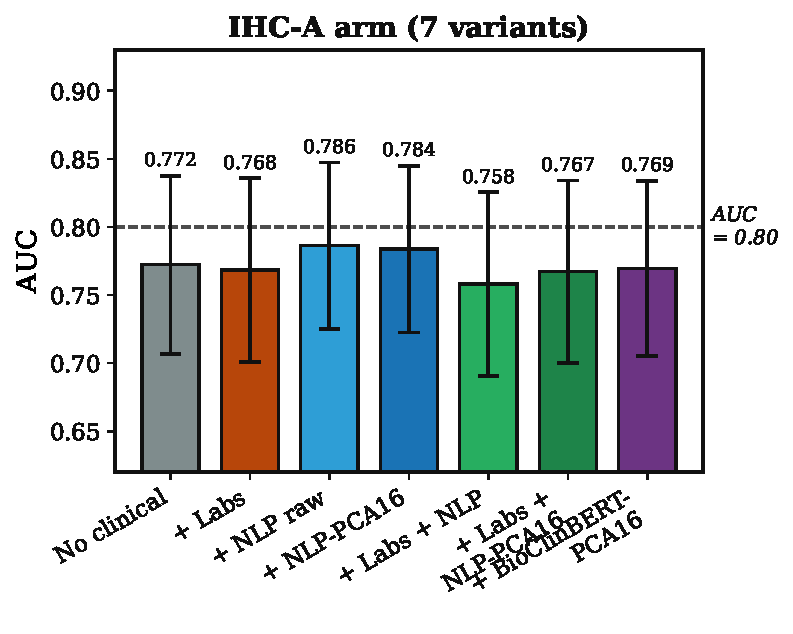
\includegraphics[width=0.48\textwidth]{figures/fig3a_auc_ihca_demo.pdf}}
  \hfill
  \subfloat[IHC-G arm (4 variants)\label{fig:auc_ihcg}]{%
    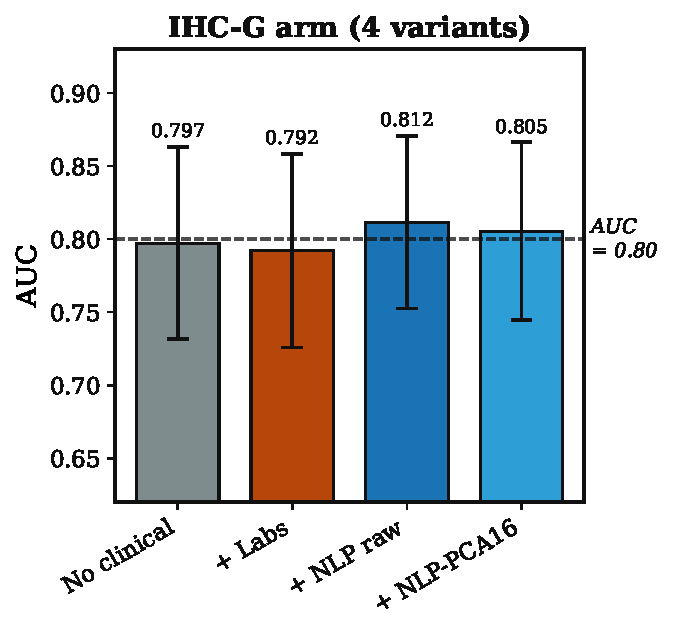
\includegraphics[width=0.48\textwidth]{figures/fig3b_auc_ihcg_demo.pdf}}
  \caption{AUC comparison across clinical encoding strategies for
    (\textbf{A}) the IHC-A arm and (\textbf{B}) the IHC-G arm. Bars show
    the AUC of a single 10-fold cross-validation partition ($n = 247$); error
    bars denote the DeLong 95\% confidence interval. The
    dashed horizontal line at AUC~$=0.80$ marks the conventional threshold
    for clinically useful discrimination.}
  \label{fig:auc_comparison}
\end{figure}

\subsection{OvO Competitive Attention with NLP Encoding Gives the Highest Fusion AUC with a Simpler Parameterization}
\label{sec:ovo}

We compared the OvO attention variant with the original cooperative attention across the 21 modality
combinations of the primary paper-matched configuration set, without and with the NLP-clinical encoding
of Section~\ref{sec:nlp_auc} (Table~\ref{tab:ovo_all21}).
Because a cohort of 247 patients cannot support reliable hypothesis tests of differences of this size,
we report the difference in AUC and the number of configurations favouring each model; we do not use
significance testing to claim superiority.

Without NLP, the largest gains for OvO over the cooperative model were for TMB+PDL1 ($\Delta\text{AUC} = +6.29\%$, AUC 0.699 vs.\ 0.636) and PDL1+Gen
($+2.27\%$, 0.716 vs.\ 0.693; Table~\ref{tab:ovo}); the cooperative model was higher for IHC-G+Gen ($-3.27\%$)
and Rad+IHC-A+Gen+PDL1 ($-3.03\%$).
At the primary benchmark (Rad+IHC-G+Gen+PDL1, BM1), OvO reached an AUC of $0.801$ (95\% CI 0.735--0.866)
versus $0.783$ (0.714--0.853) for the cooperative model ($\Delta\text{AUC} = +0.017$).

Only the two configurations that contain numeric labs (rows 20 and 21) have an NLP counterpart in
Table~\ref{tab:ovo_all21}, because the NLP encoding replaces the labs source; the remaining configurations contain no
clinical information, so their +NLP entries simply repeat the values without NLP.
In the labs-replaced configuration of BM2 (Rad+IHC-G+Gen+PDL1 with NLP), DyAM+NLP reached $0.803$ (0.738--0.868) and
OvO+NLP $0.824$ (0.765--0.883) ($\Delta = +0.021$); the intervals overlap almost completely.
Relative to BM1, which has the same sources without any clinical variable, the NLP gain was $+0.020$ for DyAM and
$+0.024$ for OvO.
OvO+NLP reached the highest AUC in this study ($0.824$), against $0.803$ for DyAM+NLP and $0.798$ for
the cooperative model without NLP (Rad+IHC-A+Gen+PDL1, the primary result of the original publication, which
this evaluation reproduced).

OvO's potential advantage is plausibly one of parameter economy: with the 384-dimensional NLP source
in the BM2 configuration, the cooperative model has 4{,}969 trainable parameters against 1{,}242 for OvO.
We did not test this explanation directly; for example, we did not shrink the cooperative attention matrix
to see whether the gap closes.
Table~\ref{tab:ovo} gives the largest single-configuration differences and Table~\ref{tab:ovo_all21} the AUC
of both attention mechanisms, with and without NLP, across all 21 configurations.

\begin{table}[H]
\caption{Largest differences between OvO competitive attention and original cooperative attention among the
  21 configurations, from a single 10-fold partition.
  $\Delta$AUC is computed as OvO minus Original.
  The upper block lists configurations in which OvO was higher, the lower block those in which the original was higher.
  Bold denotes the higher AUC for each row.
  Differences from one partition can favour either model by chance.
  Gen, genomics; Rad, CT radiomics; IHC-A/G, immunohistochemistry variants;
  PDL1, PD-L1 TPS score.}
\label{tab:ovo}
\centering
\footnotesize
\begin{tabular}{@{}lccc@{}}
\toprule
Configuration & Orig. & OvO & $\Delta$ \\
\midrule
TMB+PDL1                & 0.636 & \textbf{0.699} & +6.29\% \\
PDL1+Gen                & 0.693 & \textbf{0.716} & +2.27\% \\
Rad+IHC-G+Gen+PDL1      & 0.783 & \textbf{0.801} & +1.71\% \\
Rad+IHC-G+Gen+PDL1+Labs & 0.781 & \textbf{0.794} & +1.22\% \\
Rad+IHC-A+Gen+TMB+PDL1  & 0.778 & \textbf{0.780} & +0.24\% \\
\midrule
Rad+IHC-G               & \textbf{0.713} & 0.702 & $-1.10\%$ \\
Rad-LU                  & \textbf{0.699} & 0.684 & $-1.53\%$ \\
Rad+IHC-A+MutAmp        & \textbf{0.782} & 0.767 & $-1.54\%$ \\
Rad+IHC-A+Gen+PDL1      & \textbf{0.798} & 0.768 & $-3.03\%$ \\
IHC-G+Gen               & \textbf{0.756} & 0.723 & $-3.27\%$ \\
\bottomrule
\end{tabular}
\end{table}

%% tables/table_ovo_all21.tex  (GENERATED by make_tables_single.py - do not edit by hand)
\begin{table}[H]
\centering
\caption{AUC across all 21 paper-matched modality combinations for cooperative attention (DyAM) and OvO
  competitive attention, each without and with NLP-clinical encoding, from a single 10-fold
  cross-validation partition (natural patient order, the protocol of the original DyAM publication;
  $n = 247$). $k$ is the number of fused input sources (CT radiomics contributes one source per lesion
  site). For $k = 1$ OvO reduces algebraically to the
  cooperative formulation, hence the identical values. Configurations 8, 11, 18 and 21 are the primary
  benchmarks BM4, BM3, BM1 and BM2. The NLP encoding replaces the numeric labs source, so only the two configurations that contain labs (20 and 21) differ between the models with and without NLP; the other configurations contain no clinical source, and their +NLP values repeat those of the models without NLP (not in bold). Bold marks the highest value in each row.}
\label{tab:ovo_all21}
\footnotesize
\begin{tabular}{@{}rlcrrrr@{}}
\toprule
\# & Configuration & $k$ & DyAM & OvO & DyAM+NLP & OvO+NLP \\
\midrule
1  & TMB                              & 1 & \textbf{0.615} & \textbf{0.615} & 0.615 & 0.615 \\
2  & PDL1                             & 1 & \textbf{0.708} & \textbf{0.708} & 0.708 & 0.708 \\
3  & IHC-A                            & 1 & \textbf{0.606} & \textbf{0.606} & 0.606 & 0.606 \\
4  & Gen                              & 1 & \textbf{0.676} & \textbf{0.676} & 0.676 & 0.676 \\
5  & Rad                              & 3 & \textbf{0.701} & 0.700 & 0.701 & 0.700 \\
6  & Rad-LU                           & 4 & \textbf{0.699} & 0.684 & 0.699 & 0.684 \\
7  & TMB+PDL1                         & 2 & 0.636 & \textbf{0.699} & 0.636 & 0.699 \\
8  & PDL1+Gen (BM4)                   & 2 & 0.693 & \textbf{0.716} & 0.693 & 0.716 \\
9  & Rad+IHC-A                        & 4 & \textbf{0.681} & 0.672 & 0.681 & 0.672 \\
10 & Rad+IHC-G                        & 4 & \textbf{0.713} & 0.702 & 0.713 & 0.702 \\
11 & Rad+Gen (BM3)                    & 4 & \textbf{0.759} & 0.755 & 0.759 & 0.755 \\
12 & IHC-A+Gen                        & 2 & 0.715 & \textbf{0.716} & 0.715 & 0.716 \\
13 & IHC-G+Gen                        & 2 & \textbf{0.756} & 0.723 & 0.756 & 0.723 \\
14 & Rad+IHC-A+Gen                    & 5 & \textbf{0.754} & 0.748 & 0.754 & 0.748 \\
15 & Rad+IHC-G+Gen                    & 5 & \textbf{0.782} & 0.774 & 0.782 & 0.774 \\
16 & Rad+IHC-A+MutAmp                 & 6 & \textbf{0.782} & 0.767 & 0.782 & 0.767 \\
17 & Rad+IHC-A+Gen+PDL1               & 6 & \textbf{0.798} & 0.768 & 0.798 & 0.768 \\
18 & Rad+IHC-G+Gen+PDL1 (BM1)         & 6 & 0.783 & \textbf{0.801} & 0.783 & 0.801 \\
19 & Rad+IHC-A+Gen+TMB+PDL1           & 7 & 0.778 & \textbf{0.780} & 0.778 & 0.780 \\
20 & Rad+IHC-A+Gen+PDL1+Labs          & 7 & 0.753 & 0.749 & 0.772 & \textbf{0.782} \\
21 & Rad+IHC-G+Gen+PDL1+Labs (BM2)    & 7 & 0.781 & 0.794 & 0.803 & \textbf{0.824} \\
\bottomrule
\end{tabular}
\end{table}


%% ═══════════════════════════════════════════════════════════════════════════
%% B9 — Survival Analysis
%% ═══════════════════════════════════════════════════════════════════════════

\subsection{Survival Analysis Across the 21 Configurations}
\label{sec:survival}

For every one of the 21 configurations of Table~\ref{tab:ovo_all21} we evaluated the association of the out-of-fold risk score with
progression-free survival (PFS) in the same single partition, with the same models (DyAM and OvO, and their +NLP versions in the two
configurations that contain labs): Harrell's C-index and the multivariate Cox hazard ratio, adjusted for age, ECOG performance status,
serum albumin, dNLR and liver metastasis status (Table~\ref{tab:survival}), the log-rank $\chi^2$ at the median risk score and the
time-dependent AUC (Table~\ref{tab:km}, Figure~\ref{fig:survival_summary}; the 6- and 18-month values are in the Supplementary Tables).

\paragraph{Survival association grows with the number of fused sources.}
Single-source scores had a C-index of $0.56$--$0.59$ and a 12-month time-dependent AUC of $0.58$--$0.66$ (TMB, PD-L1, IHC-A, genomics),
and the log-rank $\chi^2$ was $1.9$ for IHC-A and $6.1$--$16.8$ for the other three.
With six or seven fused sources the C-index was $0.59$--$0.66$, the 12-month time-dependent AUC $0.69$--$0.77$, the hazard ratio per unit of
risk score $4.4$--$8.6$, and the log-rank $\chi^2$ $12.1$--$33.0$, all above the $p < 0.005$ threshold of $7.88$.
The strongest association among all configurations was obtained by cooperative attention at Rad+IHC-A+Gen+PDL1 (configuration~17;
C-index $0.655$, hazard ratio $8.59$, $\chi^2 = 33.0$, 12-month time-dependent AUC $0.774$), the configuration in which the
cooperative model also had its highest AUC.

\paragraph{OvO attention with the NLP encoding at the primary benchmarks.}
At BM1 (Rad+IHC-G+Gen+PDL1, configuration~18), OvO had a higher hazard ratio ($5.83$ against $5.27$) and log-rank $\chi^2$
($20.3$ against $17.4$) than cooperative attention, and OvO with the NLP encoding reached the highest values of the four models
in the labs-replaced configuration of BM2 (configuration~21: hazard ratio $6.64$ against $4.63$, $5.17$ and $6.13$ for DyAM, DyAM+NLP and OvO;
$\chi^2 = 23.9$ against $17.6$, $19.2$ and $20.9$), with a 12-month time-dependent AUC of $0.733$ against $0.698$, $0.702$ and $0.709$
and an 18-month value of $0.690$ against $0.650$ for DyAM+NLP.
In configuration~20 (IHC-A in place of IHC-G) the same ordering held for the hazard ratio ($6.60$ for OvO with NLP, against $4.70$, $5.80$ and $5.44$).
The C-index did not follow this order ($0.633$ for OvO with NLP and $0.646$ for DyAM at BM1), so the higher hazard ratio reflects stronger separation of
the risk groups rather than better ranking of patients.
Across the other configurations the survival metrics of the two attention mechanisms were close, each being higher in some rows
(Tables~\ref{tab:survival} and~\ref{tab:km}); OvO had the higher hazard ratio at, for example, PDL1+Gen (configuration~8: $3.01$ against $2.70$), Rad+Gen
($5.00$ against $4.74$), TMB+PDL1 ($3.00$ against $2.17$) and Rad+IHC-A+Gen+TMB+PDL1 ($7.04$ against $4.88$).

\paragraph{Kaplan--Meier curves.}
Figure~\ref{fig:km_curves} shows the curves at BM1 for the four models; the high- and low-risk groups separated in all four
(log-rank $\chi^2 = 17.4$, $20.3$, $19.2$ and $23.9$ for DyAM, OvO, DyAM+NLP and OvO+NLP).

\paragraph{Clinical encodings in the two pathology arms.}
The comparison of clinical encodings (no clinical information, numeric labs, NLP raw, NLP-PCA16, and Bio\_ClinicalBERT) in the IHC-A and IHC-G arms
(Supplementary Tables and Figures) gave hazard ratios of $5.0$--$6.3$, C-indices of $0.62$--$0.64$ and log-rank $\chi^2$ above $17$ for every variant,
with no consistent ordering of the encodings; numeric labs gave the highest C-index in both arms (IHC-A: $0.631$ against $0.623$ for NLP raw;
IHC-G: $0.644$ against $0.627$).
The NLP encoding therefore matched numeric labs on these survival metrics, and its advantage in this study is on the response endpoint (Section~\ref{sec:nlp_auc}).

%% tables/table_surv21a.tex  (GENERATED by make_surv21_tables.py - do not edit by hand)
\begin{table}[H]
\centering
\caption{Progression-free survival association of the fused risk score across the 21 configurations: Harrell's C-index and the Cox hazard ratio per unit of risk score (adjusted for age, ECOG, albumin, dNLR and liver metastases). Single 10-fold partition (natural patient order, $n = 247$; 209 events, median PFS 2.7~months), the same models and partition as Table~\ref{tab:ovo_all21}. As there, the NLP encoding replaces the numeric labs, so only configurations 20 and 21 differ between the models with and without NLP; the +NLP entries of the other configurations repeat the values without NLP (not in bold). For $k = 1$ OvO reduces to the cooperative formulation. Bold marks the highest value in each row and metric. }
\label{tab:survival}
\scriptsize
\setlength{\tabcolsep}{2pt}
\begin{tabular}{@{}rlccccccccc@{}}
\toprule
 & & & \multicolumn{4}{c}{C-index} & \multicolumn{4}{c}{Cox HR} \\
\cmidrule(lr){4-7} \cmidrule(lr){8-11}
\# & Configuration & $k$ & DyAM & OvO & DyAM+NLP & OvO+NLP & DyAM & OvO & DyAM+NLP & OvO+NLP \\
\midrule
1  & TMB                            & 1 & \textbf{0.566} & \textbf{0.566} & 0.566 & 0.566 & \textbf{3.67} & \textbf{3.67} & 3.67 & 3.67 \\
2  & PDL1                           & 1 & \textbf{0.580} & \textbf{0.580} & 0.580 & 0.580 & \textbf{2.15} & \textbf{2.15} & 2.15 & 2.15 \\
3  & IHC-A                          & 1 & \textbf{0.555} & \textbf{0.555} & 0.555 & 0.555 & \textbf{1.93} & \textbf{1.93} & 1.93 & 1.93 \\
4  & Gen                            & 1 & \textbf{0.586} & \textbf{0.586} & 0.586 & 0.586 & \textbf{3.28} & \textbf{3.28} & 3.28 & 3.28 \\
5  & Rad                            & 3 & \textbf{0.582} & 0.577 & 0.582 & 0.577 & \textbf{2.82} & 2.79 & 2.82 & 2.79 \\
6  & Rad-LU                         & 4 & 0.566 & \textbf{0.569} & 0.566 & 0.569 & 2.91 & \textbf{2.99} & 2.91 & 2.99 \\
7  & TMB+PDL1                       & 2 & 0.564 & \textbf{0.582} & 0.564 & 0.582 & 2.17 & \textbf{3.00} & 2.17 & 3.00 \\
8  & PDL1+Gen (BM4)                 & 2 & 0.589 & \textbf{0.602} & 0.589 & 0.602 & 2.70 & \textbf{3.01} & 2.70 & 3.01 \\
9  & Rad+IHC-A                      & 4 & 0.584 & \textbf{0.585} & 0.584 & 0.585 & \textbf{2.71} & 2.65 & 2.71 & 2.65 \\
10 & Rad+IHC-G                      & 4 & \textbf{0.591} & 0.586 & 0.591 & 0.586 & \textbf{2.76} & 2.71 & 2.76 & 2.71 \\
11 & Rad+Gen (BM3)                  & 4 & 0.605 & \textbf{0.609} & 0.605 & 0.609 & 4.74 & \textbf{5.00} & 4.74 & 5.00 \\
12 & IHC-A+Gen                      & 2 & 0.603 & \textbf{0.608} & 0.603 & 0.608 & 3.59 & \textbf{3.75} & 3.59 & 3.75 \\
13 & IHC-G+Gen                      & 2 & \textbf{0.622} & 0.612 & 0.622 & 0.612 & \textbf{4.04} & 3.59 & 4.04 & 3.59 \\
14 & Rad+IHC-A+Gen                  & 5 & \textbf{0.619} & \textbf{0.619} & 0.619 & 0.619 & \textbf{5.68} & 5.45 & 5.68 & 5.45 \\
15 & Rad+IHC-G+Gen                  & 5 & \textbf{0.630} & 0.628 & 0.630 & 0.628 & \textbf{5.42} & 4.83 & 5.42 & 4.83 \\
16 & Rad+IHC-A+MutAmp               & 6 & \textbf{0.621} & 0.592 & 0.621 & 0.592 & \textbf{4.70} & 4.40 & 4.70 & 4.40 \\
17 & Rad+IHC-A+Gen+PDL1             & 6 & \textbf{0.655} & 0.620 & 0.655 & 0.620 & \textbf{8.59} & 6.29 & 8.59 & 6.29 \\
18 & Rad+IHC-G+Gen+PDL1 (BM1)       & 6 & \textbf{0.646} & 0.640 & 0.646 & 0.640 & 5.27 & \textbf{5.83} & 5.27 & 5.83 \\
19 & Rad+IHC-A+Gen+TMB+PDL1         & 7 & \textbf{0.624} & 0.620 & 0.624 & 0.620 & 4.88 & \textbf{7.04} & 4.88 & 7.04 \\
20 & Rad+IHC-A+Gen+PDL1+Labs        & 7 & \textbf{0.625} & 0.619 & 0.621 & 0.621 & 4.70 & 5.44 & 5.80 & \textbf{6.60} \\
21 & Rad+IHC-G+Gen+PDL1+Labs (BM2)  & 7 & \textbf{0.640} & 0.637 & 0.630 & 0.633 & 4.63 & 6.13 & 5.17 & \textbf{6.64} \\
\bottomrule
\end{tabular}
\end{table}

%% tables/table_surv21b.tex  (GENERATED by make_surv21_tables.py - do not edit by hand)
\begin{table}[H]
\centering
\caption{Kaplan--Meier log-rank statistic (patients dichotomised at the median risk score; $\chi^2 > 3.84$ corresponds to $p < 0.05$) and cumulative/dynamic time-dependent AUC at 12 months (Uno estimator) across the 21 configurations. Single 10-fold partition (natural patient order, $n = 247$; 209 events, median PFS 2.7~months), the same models and partition as Table~\ref{tab:ovo_all21}. As there, the NLP encoding replaces the numeric labs, so only configurations 20 and 21 differ between the models with and without NLP; the +NLP entries of the other configurations repeat the values without NLP (not in bold). For $k = 1$ OvO reduces to the cooperative formulation. Bold marks the highest value in each row and metric. Time-dependent AUC at 6 and 18 months is in the Supplementary Tables.}
\label{tab:km}
\scriptsize
\setlength{\tabcolsep}{2pt}
\begin{tabular}{@{}rlccccccccc@{}}
\toprule
 & & & \multicolumn{4}{c}{Log-rank $\chi^2$} & \multicolumn{4}{c}{tdAUC 12~mo} \\
\cmidrule(lr){4-7} \cmidrule(lr){8-11}
\# & Configuration & $k$ & DyAM & OvO & DyAM+NLP & OvO+NLP & DyAM & OvO & DyAM+NLP & OvO+NLP \\
\midrule
1  & TMB                            & 1 & \textbf{8.5} & \textbf{8.5} & 8.5 & 8.5 & \textbf{0.596} & \textbf{0.596} & 0.596 & 0.596 \\
2  & PDL1                           & 1 & \textbf{16.8} & \textbf{16.8} & 16.8 & 16.8 & \textbf{0.662} & \textbf{0.662} & 0.662 & 0.662 \\
3  & IHC-A                          & 1 & \textbf{1.9} & \textbf{1.9} & 1.9 & 1.9 & \textbf{0.577} & \textbf{0.577} & 0.577 & 0.577 \\
4  & Gen                            & 1 & \textbf{6.1} & \textbf{6.1} & 6.1 & 6.1 & \textbf{0.661} & \textbf{0.661} & 0.661 & 0.661 \\
5  & Rad                            & 3 & 5.0 & \textbf{7.3} & 5.0 & 7.3 & \textbf{0.651} & 0.646 & 0.651 & 0.646 \\
6  & Rad-LU                         & 4 & 3.7 & \textbf{7.6} & 3.7 & 7.6 & \textbf{0.612} & 0.603 & 0.612 & 0.603 \\
7  & TMB+PDL1                       & 2 & 11.6 & \textbf{20.8} & 11.6 & 20.8 & 0.589 & \textbf{0.617} & 0.589 & 0.617 \\
8  & PDL1+Gen (BM4)                 & 2 & 18.8 & \textbf{20.8} & 18.8 & 20.8 & 0.630 & \textbf{0.654} & 0.630 & 0.654 \\
9  & Rad+IHC-A                      & 4 & 11.2 & \textbf{13.8} & 11.2 & 13.8 & 0.613 & \textbf{0.642} & 0.613 & 0.642 \\
10 & Rad+IHC-G                      & 4 & \textbf{13.9} & 13.3 & 13.9 & 13.3 & \textbf{0.636} & 0.623 & 0.636 & 0.623 \\
11 & Rad+Gen (BM3)                  & 4 & \textbf{20.5} & 20.2 & 20.5 & 20.2 & 0.715 & \textbf{0.730} & 0.715 & 0.730 \\
12 & IHC-A+Gen                      & 2 & \textbf{20.9} & 16.5 & 20.9 & 16.5 & 0.654 & \textbf{0.658} & 0.654 & 0.658 \\
13 & IHC-G+Gen                      & 2 & \textbf{18.7} & 16.0 & 18.7 & 16.0 & \textbf{0.644} & 0.618 & 0.644 & 0.618 \\
14 & Rad+IHC-A+Gen                  & 5 & 16.8 & \textbf{17.3} & 16.8 & 17.3 & 0.695 & \textbf{0.718} & 0.695 & 0.718 \\
15 & Rad+IHC-G+Gen                  & 5 & \textbf{15.6} & 13.5 & 15.6 & 13.5 & 0.698 & \textbf{0.705} & 0.698 & 0.705 \\
16 & Rad+IHC-A+MutAmp               & 6 & \textbf{20.5} & 12.9 & 20.5 & 12.9 & \textbf{0.710} & 0.694 & 0.710 & 0.694 \\
17 & Rad+IHC-A+Gen+PDL1             & 6 & \textbf{33.0} & 18.9 & 33.0 & 18.9 & \textbf{0.774} & 0.732 & 0.774 & 0.732 \\
18 & Rad+IHC-G+Gen+PDL1 (BM1)       & 6 & 17.4 & \textbf{20.3} & 17.4 & 20.3 & \textbf{0.726} & 0.717 & 0.726 & 0.717 \\
19 & Rad+IHC-A+Gen+TMB+PDL1         & 7 & \textbf{21.1} & 21.0 & 21.1 & 21.0 & 0.712 & \textbf{0.725} & 0.712 & 0.725 \\
20 & Rad+IHC-A+Gen+PDL1+Labs        & 7 & \textbf{23.3} & 12.1 & 22.1 & 20.1 & 0.690 & 0.698 & 0.693 & \textbf{0.731} \\
21 & Rad+IHC-G+Gen+PDL1+Labs (BM2)  & 7 & 17.6 & 20.9 & 19.2 & \textbf{23.9} & 0.698 & 0.709 & 0.702 & \textbf{0.733} \\
\bottomrule
\end{tabular}
\end{table}


\begin{figure}[H]
  \centering
  \subfloat[BM1, DyAM]{%
    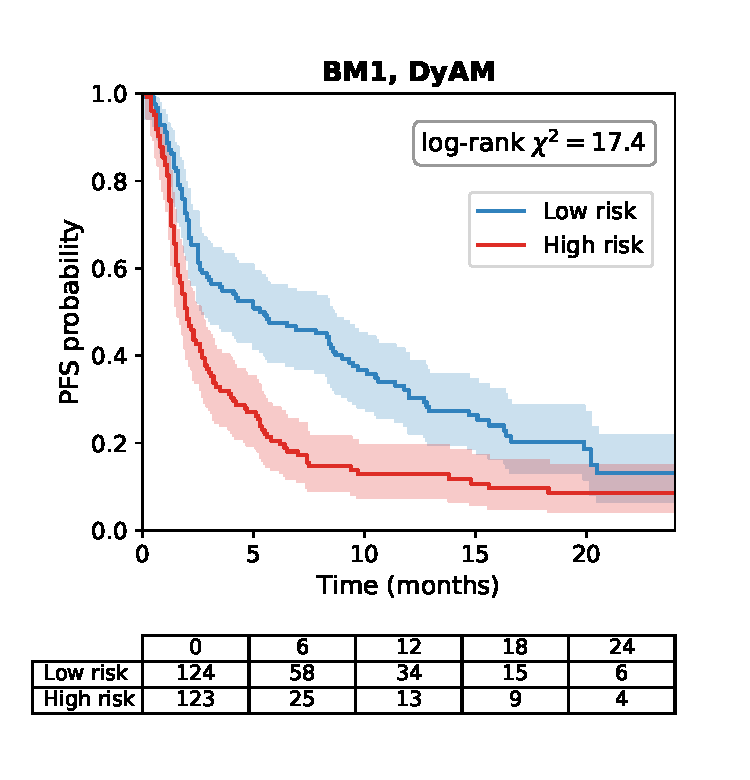
\includegraphics[width=0.48\textwidth]{figures/fig4a_km_bm1_dyam.pdf}}
  \hfill
  \subfloat[BM1, OvO]{%
    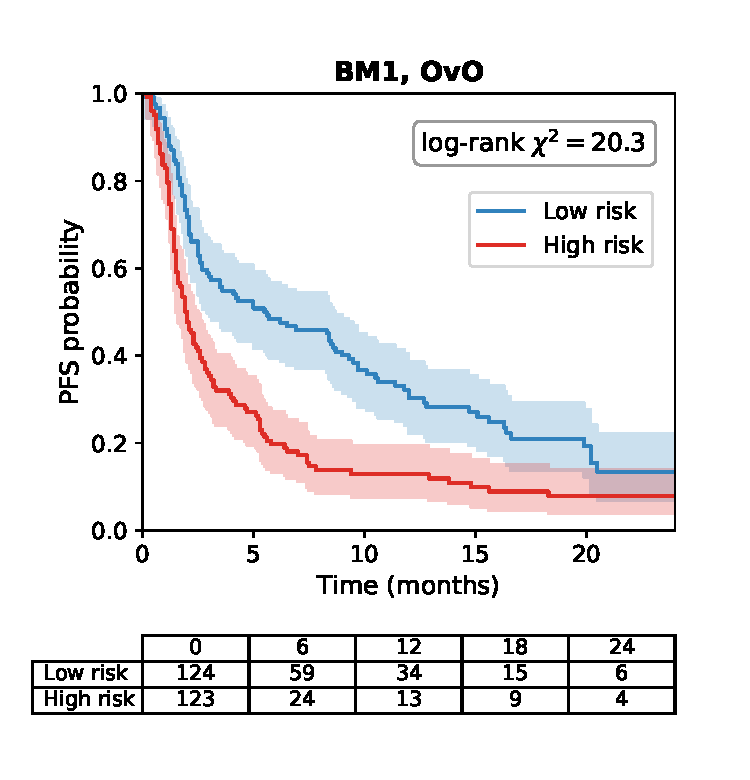
\includegraphics[width=0.48\textwidth]{figures/fig4b_km_bm1_ovo.pdf}}

  \subfloat[BM1, DyAM+NLP]{%
    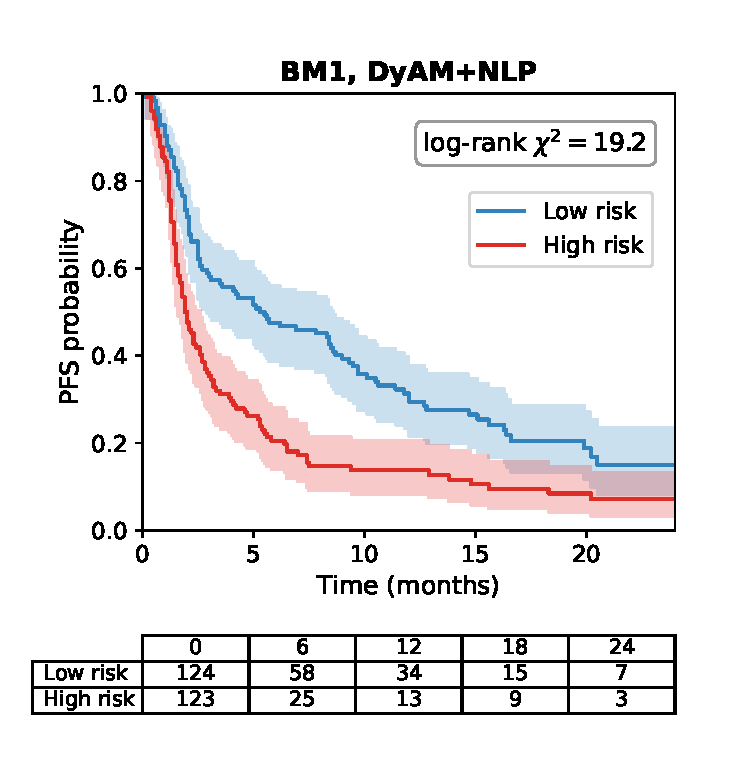
\includegraphics[width=0.48\textwidth]{figures/fig4c_km_bm1_dyam_nlp.pdf}}
  \hfill
  \subfloat[BM1, OvO+NLP]{%
    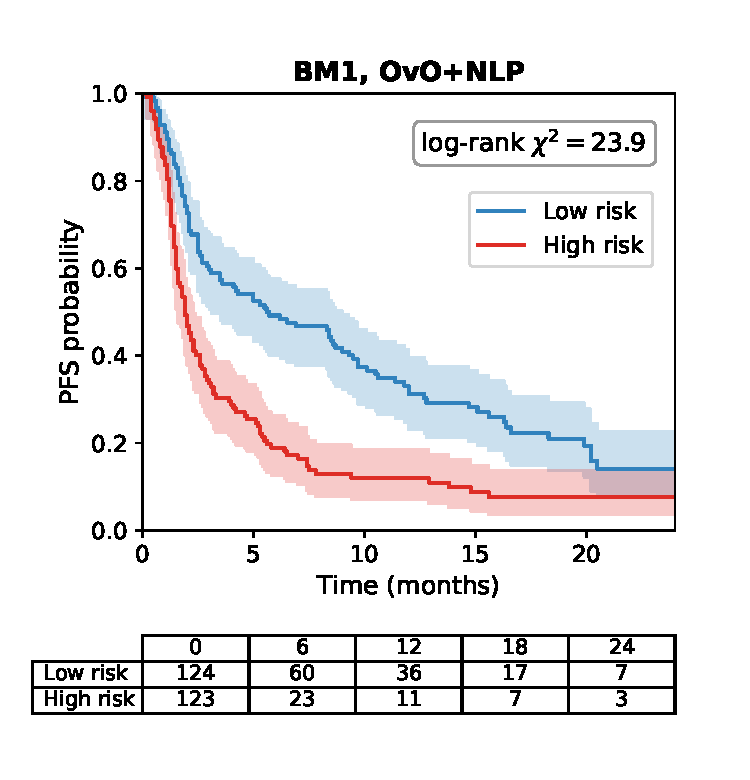
\includegraphics[width=0.48\textwidth]{figures/fig4d_km_bm1_ovo_nlp.pdf}}
  \caption{Kaplan--Meier progression-free survival curves at the primary benchmark BM1 (Rad+IHC-G+Gen+PDL1), computed from the out-of-fold risk
    scores of the single 10-fold partition and stratified at the median risk score into high-risk (red) and low-risk (blue) groups,
    with number-at-risk tables. The log-rank statistics printed in the panels are those of Table~\ref{tab:km} (BM1 rows;
    for the two +NLP panels the NLP encoding is added to the BM1 sources).
    (\textbf{A}) DyAM. (\textbf{B}) OvO. (\textbf{C}) DyAM+NLP. (\textbf{D}) OvO+NLP.}
  \label{fig:km_curves}
\end{figure}

\begin{figure}[H]
  \centering
  \subfloat[Harrell's C-index]{%
    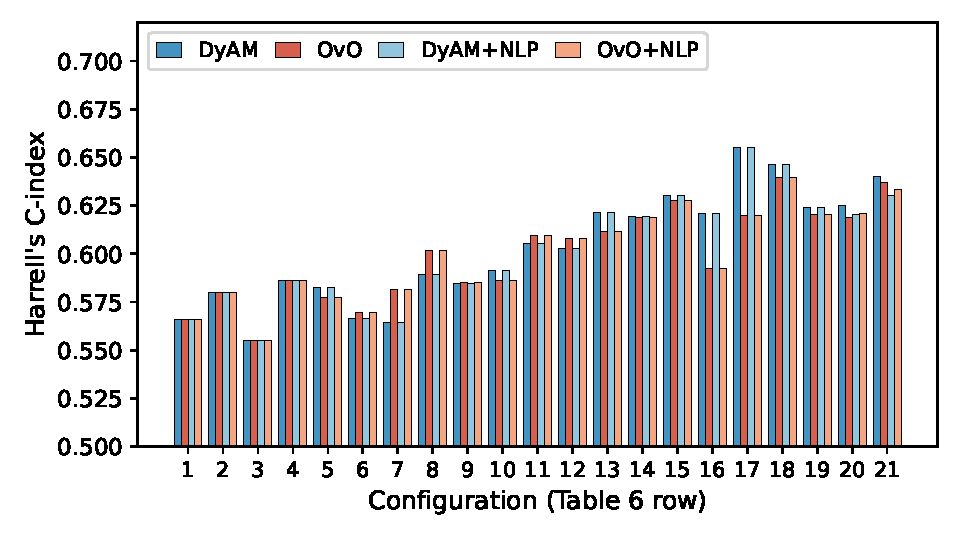
\includegraphics[width=0.48\textwidth]{figures/fig5a_cindex.pdf}}
  \hfill
  \subfloat[Time-dependent AUC at 12~months]{%
    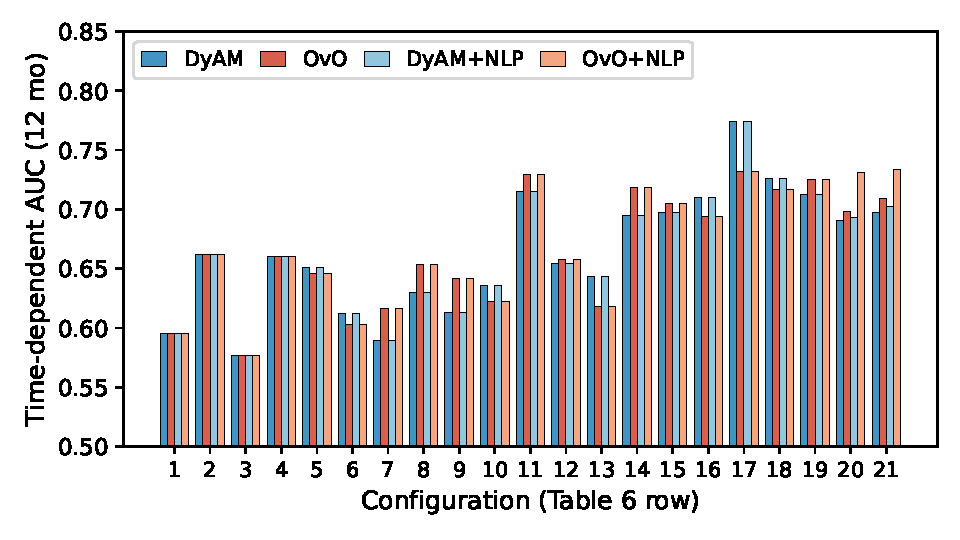
\includegraphics[width=0.48\textwidth]{figures/fig5b_tdauc.pdf}}

  \subfloat[Multivariate Cox hazard ratio]{%
    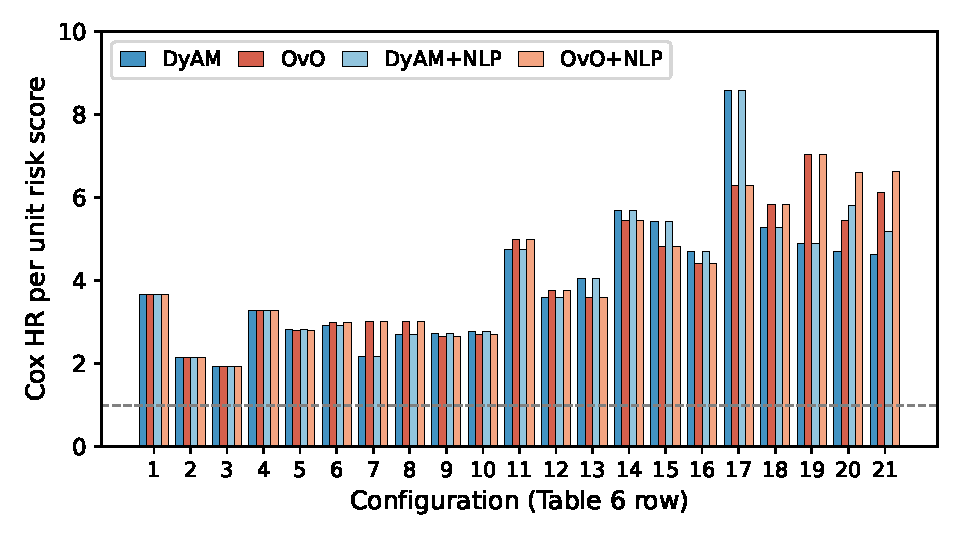
\includegraphics[width=0.48\textwidth]{figures/fig5c_cox_forest.pdf}}
  \hfill
  \subfloat[Kaplan--Meier log-rank $\chi^2$]{%
    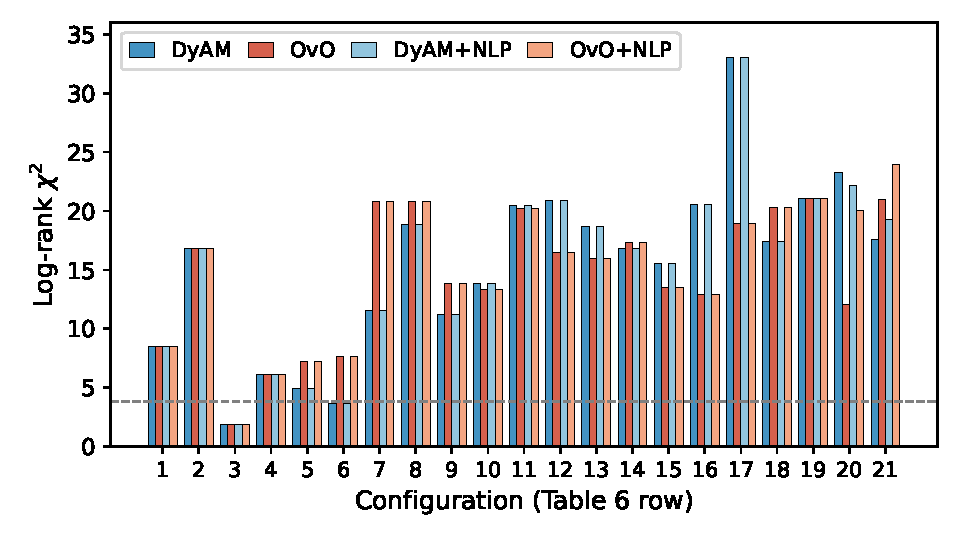
\includegraphics[width=0.48\textwidth]{figures/fig5d_km_chi2.pdf}}
  \caption{Survival association of the risk score across the 21 configurations (numbered as in Table~\ref{tab:ovo_all21}), single 10-fold partition.
    Bars show DyAM, OvO, and, where they differ (configurations 20 and 21), DyAM+NLP and OvO+NLP; for the other configurations the +NLP bars repeat the values without NLP.
    (\textbf{A}) Harrell's C-index (dashed line, 0.5).
    (\textbf{B}) Time-dependent AUC at 12 months.
    (\textbf{C}) Cox hazard ratio per unit of risk score, adjusted for age, ECOG performance status, albumin, dNLR and liver metastases (dashed line, 1).
    (\textbf{D}) Log-rank $\chi^2$ of the dichotomised risk score (dashed line, 3.84).}
  \label{fig:survival_summary}
\end{figure}
